
%!TEX program = xelatex
\documentclass[letterpaper,12pt]{exam}
\usepackage{../videoNotes}
\usepackage{xcolor}
\usepackage[dvipsnames]{xcolor}
\usepackage{soul}
\usepackage{draftwatermark}
\SetWatermarkText{DRAFT}
\SetWatermarkScale{1.5}
\SetWatermarkColor{red!20}
\newcommand{\unit}{Exam 2 Cheatsheet}
\pagestyle{headandfoot}

\begin{document}
\begin{tabular}{| c | c | c | c| c |}
 \hline
    rax & System Call & rdi & rsi & rdx \\
    \hline
    $0$ & read & file descriptor & buffer & number of bytes \\
    \hline
    $1$ & write & file descriptor & buffer & number of bytes \\
    \hline
\end{tabular}
\par
\vspace{0.5in}
The following is probably a placeholder, and it won't show up on the exam version.\\
\begin{tabular}{|c|c|c|c|}
    \hline
   function & arguments & return value & notes\\    
    \hline
    puts & char *s & size\_t length & does not count null byte \\
    \hline
    strcpy & char *dest, char *src & char *dest & dest must be big enough \\
    \hline
    strncmp & char *s1, char *s2, size\_t n & int & 0 if equal, $<$0 if s1<s2, $>$0 if s1>s2 \\
    \hline
    strncpy & char *dest, char *src, size\_t n & char *dest & dest must be big enough \\
    \hline
    strcat & char *dest, char *src & char *dest & dest must be big enough \\
    \hline
    strncat & char *dest, char *src, size\_t n & char *dest & dest must be big enough \\
    \hline
    strcmp & char *s1, char *s2 & int & 0 if equal, $<$0 if s1<s2, $>$0 if s1>s2 \\
    \hline
\end{tabular}
   \twocolumn
\begin{center}
\begin{tabular}{| c | c | c |}
    \hline
        n & $2^n$ & Other \\
        \hline
    $0$ & $ 1 $ & $8^0$ and $16^0$ \\ 
    $1$ & $ 2 $ & \  \\ 
\hline
    $2$ & $ 4 $ & \  \\ 
    $3$ & $ 8 $ & \  \\ 
\hline
    $4$ & $ 16 $ & $16^1$ \\ 
    $5$ & $ 32 $ & \  \\ 
\hline
    $6$ & $ 64 $ & \  \\ 
    $7$ & $ 128 $ & \  \\ 
\hline
    $8$ & $ 256 $ & $16^2$ \\ 
    $9$ & $ 512 $ & \  \\ 
\hline
    $10$ & $ 1024 $ & 1 Kilobyte \\ 
    $11$ & $ 2048 $ & \  \\ 
\hline
    $12$ & $ 4096 $ & $16^3$ \\ 
    $13$ & {\color{lightgray}  8092}  & \  \\ 
\hline
    $14$ &  {\color{lightgray}  16,384} & \  \\ 
    $15$ & $ 32,768 $ & \  \\ 
\hline
    $16$ &   65,536  & $16^4$ \\ 
    $17$ & {\color{lightgray} 131,082 } & \  \\ 
\hline
      $18$ &   {\color{lightgray}  262,144} & \  \\ 
    $19$ &  {\color{lightgray} 524,288 } & \  \\ 
\hline
      $20$ & 1,048,576  & $16^5$ 1 Megabyte \\  
\hline
    \end{tabular}
\end{center}
\par
\begin{center}
The counting in hex and binary is going to be on the exam itself
\end{center}

\begin{center}
\begin{tabular}{| c | c |}
 \hline
    Multiplication & Result \\
    \hline
 $16 \cdot 0 $ & $ 0 $ \\ 
 $16 \cdot 1 $ & $ 16 $ \\ 
\hline
 $16 \cdot 2 $ & $ 32 $ \\ 
 $16 \cdot 3 $ & $ 48 $ \\ 
\hline
 $16 \cdot 4 $ & $ 64 $ \\ 
 $16 \cdot 5 $ & $ 80 $ \\ 
\hline
 $16 \cdot 6 $ & $ 96 $ \\ 
 $16 \cdot 7 $ & $ 112 $ \\ 
\hline
 $16 \cdot 8 $ & $ 128 $ \\ 
 $16 \cdot 9 $ & $ 144 $ \\ 
\hline
$16 \cdot 10  (a)$ & $ 160 $ \\ 
$16 \cdot 11  (b) $ & $ 176 $ \\ 
\hline
$16 \cdot 12 $ (c) & $ 192 $ \\ 
$16 \cdot 13 $  (d) & $ 208 $ \\ 
\hline
$16 \cdot 14 $  (e)& $ 224 $ \\ 
$16 \cdot 15 $  (f) & $ 240 $ \\ 
\hline
 $16 \cdot 16 $ & $ 256 $ \\   
\hline
\end{tabular}
\end{center}

\begin{center}
    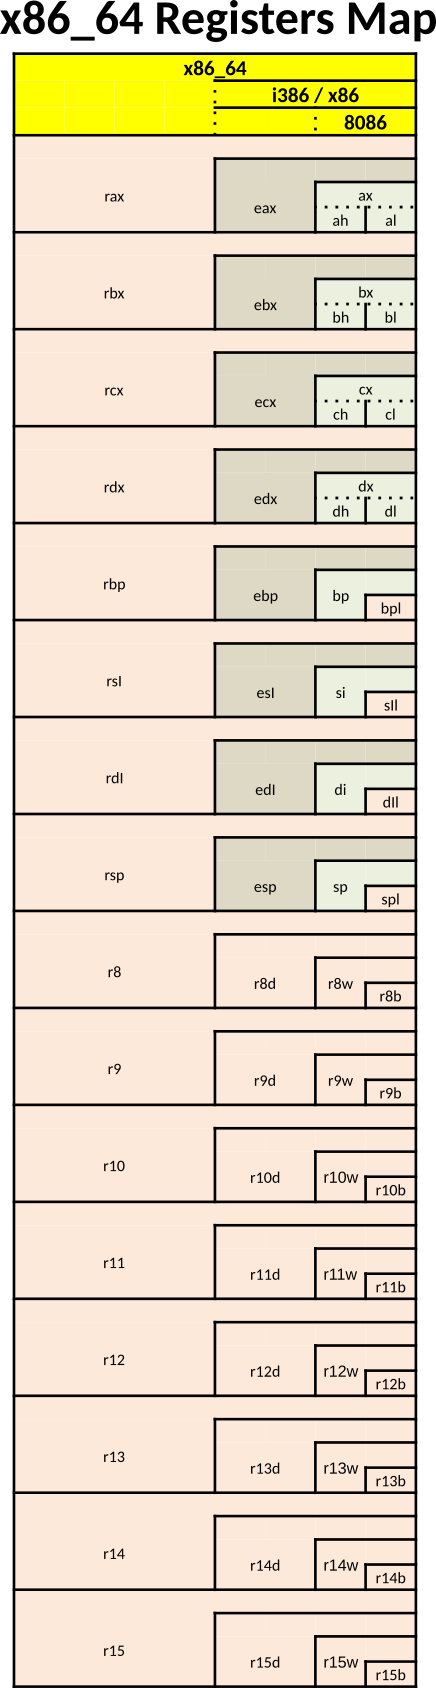
\includegraphics[height=9in]{../../02_Registers/images/X86_64-GP-registersBIG.png}
    

%\includegraphics[height=8in]{../../02}
\end{center}

\end{document} 